\documentclass[conference]{IEEEtran}
\IEEEoverridecommandlockouts
\usepackage{cite}
\usepackage{amsmath,amssymb,amsfonts}
\usepackage{graphicx}
\usepackage{booktabs}
\usepackage{textcomp}
\usepackage{xcolor}
\usepackage{url}
\usepackage[hidelinks]{hyperref}

\begin{document}

\title{Parameter-Efficient Fine-Tuning of PaliGemma\\for Remote Sensing Image Captioning}

\author{\IEEEauthorblockN{S\"uleyman Ceran}
\IEEEauthorblockA{\textit{Department of Data Informatics, METU}\\
DI 725 Assignment 3\\
suleymanceran33@gmail.com}
\thanks{Code: \url{https://github.com/sceran/paligemma3b-QLoRA-RISC-captioning}. W\&B: \url{https://wandb.ai/sceran/paligemma3b-QLoRA-RISC}, \url{https://wandb.ai/sceran/huggingface}.}}

\maketitle

\begin{abstract}
We apply QLoRA to PaliGemma-3B on the RISC remote-sensing captioning dataset, reaching CIDEr 2.21 from a zero-shot baseline of 0.25. Two ablations extend the recipe: a caption-selection strategy comparison, and a cumulative PEFT method comparison across vanilla LoRA, rsLoRA, LoRA+, and DoRA. A short exploration swaps the base to PaliGemma 2. The ablation suggests recent PEFT improvements do not stack monotonically on this domain; rsLoRA alone is the strongest single intervention at 500 steps.
\end{abstract}

\section{Introduction}

Vision-language models perform well at captioning but adapting them to specialized domains is expensive. QLoRA \cite{dettmers2023qlora} addresses this with 4-bit base-weight quantization plus low-rank adapters \cite{hu2022lora}. We apply it to PaliGemma-3B \cite{beyer2024paligemma}, a SigLIP+Gemma VLM, on the RISC dataset of 44{,}521 satellite images each with five captions. Contributions: (i) a fine-tuned model with CIDEr 2.21 (8.7$\times$ baseline), (ii) caption-selection ablation, (iii) cumulative PEFT method comparison, (iv) a brief PaliGemma 2 swap.

\section{Approach}

The dataset is split image-level (seed 42) into 37{,}843 / 2{,}226 / 4{,}452 train/val/test. One of the five captions per image is sampled per training step (\emph{random} strategy). We use \texttt{google/paligemma-3b-pt-224} with 4-bit NF4 double quantization and bf16 compute. LoRA adapters (rank 16, $\alpha{=}32$, dropout 0.05) attach to the seven attention and MLP projection modules, giving 22.6M trainable parameters (0.77\%). The main run adds rsLoRA scaling \cite{kalajdzievski2023rslora} and LoRA+ \cite{hayou2024loraplus} (16$\times$ LR on B matrices). AdamW at $10^{-4}$, batch 4 with grad accumulation 4, gradient checkpointing, 3\% warmup, 1 epoch (2{,}366 steps). Ablations share the recipe and cap at 500 steps. Metrics use pycocoevalcap (multi-reference, all five captions).

\section{Results}

\textbf{Main result (Table~\ref{tab:main}).} CIDEr improves from 0.25 to 2.21; BLEU-4 from 0.04 to 0.58. Predictions shift from generic short outputs to longer, domain-specific captions (Fig.~\ref{fig:qualitative}).

\begin{table}[t]
\centering\small
\caption{Baseline vs.\ QLoRA fine-tuned PaliGemma (500 test images).}
\label{tab:main}
\renewcommand{\arraystretch}{1.0}
\begin{tabular}{lccccc}
\toprule
& BLEU-1 & BLEU-4 & METEOR & ROUGE-L & CIDEr \\
\midrule
Baseline    & 0.329 & 0.040 & 0.095 & 0.269 & 0.253 \\
QLoRA tuned & \textbf{0.853} & \textbf{0.585} & \textbf{0.409} & \textbf{0.750} & \textbf{2.207} \\
\bottomrule
\end{tabular}
\end{table}

\textbf{Caption strategy.} At 500 steps, random sampling reaches CIDEr 1.83 (BLEU-4 0.53); picking only the first or longest caption falls to 1.42 (BLEU-4 0.47 and 0.53). Concatenating all five into one target collapses CIDEr to 0.00 because the model learns to produce over-long outputs the metric heavily penalizes.

\textbf{Cumulative PEFT ablation (Table~\ref{tab:peft}).} rsLoRA alone scores highest; rsLoRA+LoRA+ stack trails it; adding DoRA \cite{liu2024dora} recovers some ground. Two replicates of the stack (D and G) differ by 0.16 CIDEr, an empirical inter-run noise floor. Under this lens only rsLoRA marginally exceeds the noise band.

\begin{table}[t]
\centering\small
\caption{Cumulative PEFT method ablation (500 steps each).}
\label{tab:peft}
\renewcommand{\arraystretch}{1.0}
\begin{tabular}{lcc}
\toprule
Configuration & BLEU-4 & CIDEr \\
\midrule
A. Vanilla LoRA          & 0.528 & 1.932 \\
B. rsLoRA only           & 0.513 & \textbf{2.090} \\
C. LoRA+ only            & 0.514 & 1.903 \\
D. rsLoRA + LoRA+ stack  & 0.532 & 1.828 \\
E. + DoRA                & 0.530 & 1.979 \\
G. stack replicate       & 0.543 & 1.989 \\
\bottomrule
\end{tabular}
\end{table}

\textbf{PaliGemma 2.} The rsLoRA-only configuration on PaliGemma 2 3B \cite{steiner2024paligemma2} yields CIDEr 2.095 vs.\ PG1's 2.090: a tie within the noise band. PG2 zero-shot is actually worse than PG1 (CIDEr 0.172 vs.\ 0.253), but fine-tuning closes the gap.

\begin{figure}[!h]
\centering
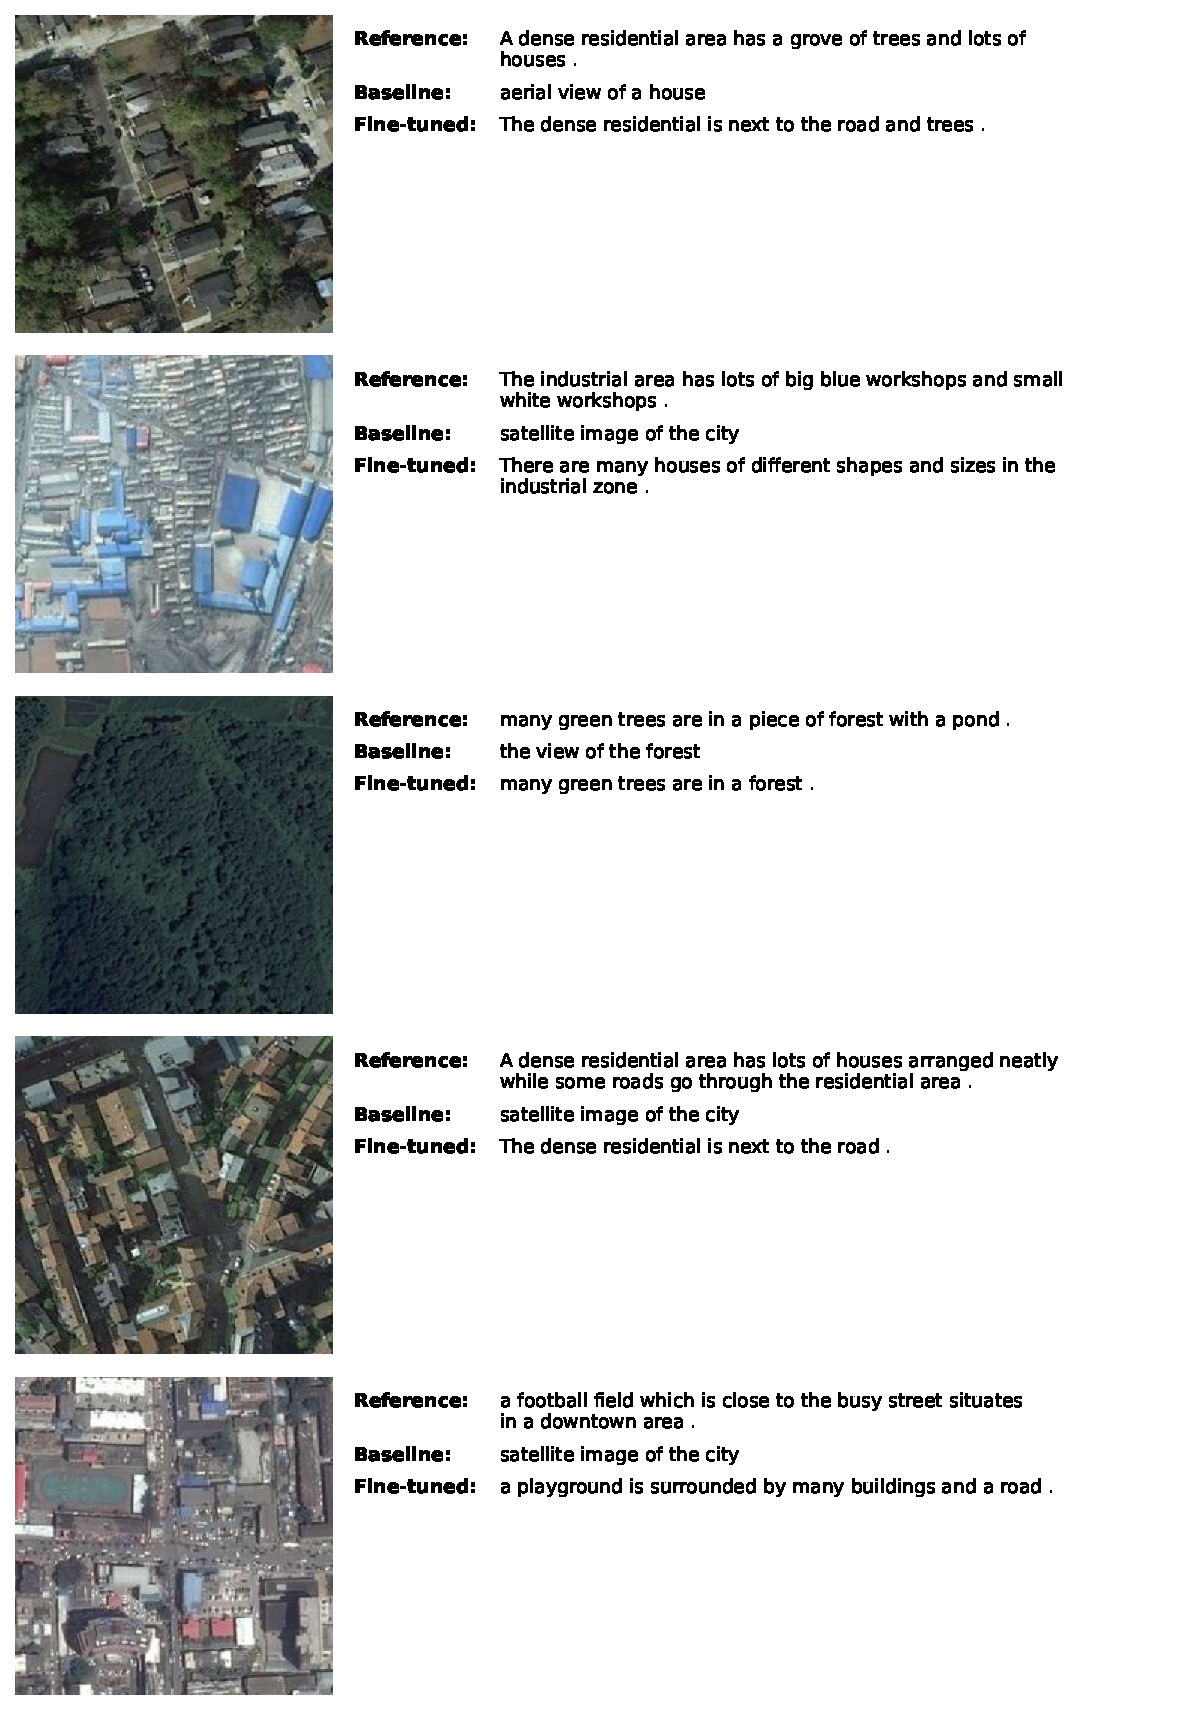
\includegraphics[width=0.65\linewidth]{qualitative.pdf}
\caption{Five test images with reference, zero-shot baseline, and fine-tuned predictions. The baseline frequently falls back to generic phrasing (``satellite image of the city'', ``aerial view of a house''), while the fine-tuned model produces RISC-style descriptions using domain vocabulary like ``residential'', ``industrial'', ``forest'', and ``playground''.}
\label{fig:qualitative}
\end{figure}

\section{Discussion and Conclusion}

Modern PEFT improvements do not stack monotonically on RISC at this budget; with a 0.16 CIDEr noise floor from our replicates, vanilla LoRA stays competitive. The base-model swap alone does not buy quality: PG2 ties PG1 at a fixed budget, and the 1-epoch PG1 main run remains ahead of the 500-step PG2 run, so training duration outweighs v1$\to$v2. QLoRA delivered an 8.7$\times$ CIDEr gain with under 1\% of the model trainable. Future work: full-epoch PG2, the instruction-tuned PG2 variant, and activation-driven initializations (EVA, CorDA) once their VLM paths stabilize.

\begin{thebibliography}{9}
\footnotesize
\bibitem{hu2022lora} E.\ J.\ Hu et al., ``LoRA: Low-rank adaptation of large language models,'' \emph{ICLR}, 2022.
\bibitem{dettmers2023qlora} T.\ Dettmers et al., ``QLoRA: Efficient finetuning of quantized LLMs,'' \emph{NeurIPS}, 2023.
\bibitem{beyer2024paligemma} L.\ Beyer et al., ``PaliGemma: A versatile 3B VLM for transfer,'' \emph{arXiv:2407.07726}, 2024.
\bibitem{steiner2024paligemma2} A.\ Steiner et al., ``PaliGemma 2,'' \emph{arXiv:2412.03555}, 2024.
\bibitem{kalajdzievski2023rslora} D.\ Kalajdzievski, ``A rank stabilization scaling factor for LoRA,'' \emph{arXiv:2312.03732}, 2023.
\bibitem{hayou2024loraplus} S.\ Hayou et al., ``LoRA+,'' \emph{ICML}, 2024.
\bibitem{liu2024dora} S.\ Liu et al., ``DoRA: Weight-decomposed low-rank adaptation,'' \emph{ICML}, 2024.
\end{thebibliography}

\end{document}
